\subsection{Phase Noise Puzzles: The Impact on SDR Performance!}

\begin{tcolorbox}[colback=gray!10, colframe=black, title=E4C01]  
What is an effect of excessive phase noise in an SDR receiver’s master clock oscillator?  
\begin{enumerate}[label=\Alph*.]
    \item It limits the receiver’s ability to receive strong signals
    \item It can affect the receiver’s frequency calibration
    \item It decreases the receiver’s third-order intercept point
    \item \textbf{It can combine with strong signals on nearby frequencies to generate interference}
\end{enumerate} \end{tcolorbox}

\subsubsection{Related Concepts}

Phase noise refers to the rapid, short-term variations in the phase of a signal. In software-defined radio (SDR) systems, the master clock oscillator plays a crucial role in determining the quality of the received signals. Excessive phase noise can lead to significant issues, particularly in scenarios where signals are close in frequency.

Understanding the impact of phase noise requires some familiarity with the concepts of modulation, signal interference, and frequency stability. When the phase noise is excessive, it results in a widening of the spectral lines of the transmitted signals, making it difficult for the receiver to distinguish between closely spaced frequencies. This can lead to a phenomenon known as interference, which occurs when two or more signals overlap and create distortions in the perceived signal.

\subsubsection{Calculating the Impact of Phase Noise}

Excessive phase noise can be analyzed using techniques from signal processing. If we denote the phase noise as \( \phi(t) \), the mathematical model of the received signal can be expressed as:

\[
s(t) = A \cos(2 \pi f_c t + \phi(t))
\]

where \( A \) is the amplitude, and \( f_c \) is the carrier frequency. The noise affects the total power of the signal, which can be quantified using the power spectral density (PSD) of the phase noise, \( S_{phi}(f) \). The effect on signal power can often be calculated using the formula:

\[
P = \int_{-\infty}^{\infty} S_{signal}(f) df 
\]

When phase noise is introduced, due to broadening of the spectral lines, the signal power becomes affected as well, and this can lead to a significant increase in the noise floor.

\subsubsection{Visual Representation}

To illustrate the concept of phase noise and its impact, we can use a diagram created with TikZ. The following diagram depicts the spectral broadening caused by excessive phase noise, leading to signal interference:

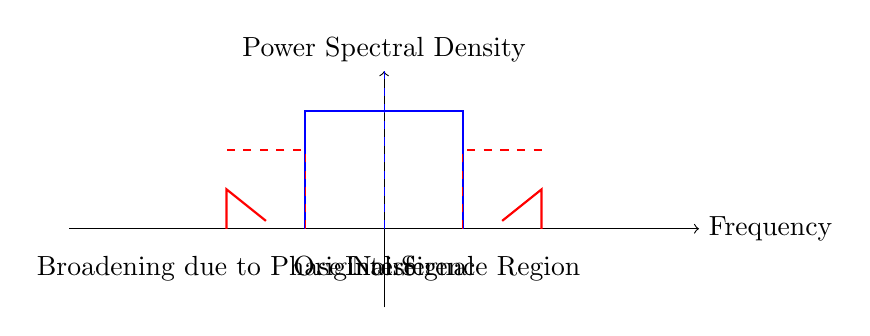
\begin{tikzpicture}
    \draw[->] (-4,0) -- (4,0) node[right] {Frequency};
    \draw[->] (0,-1) -- (0,2) node[above] {Power Spectral Density};

    % Main signal
    \draw[thick, blue] (-1,0) -- (-1,1.5) -- (1,1.5) -- (1,0);
    \draw[dashed, blue] (0,0) -- (0,2); % Peak power line

    % Phase noise effect
    \draw[thick, red] (-2,0) -- (-2,0.5) -- (-1.5,0.1);
    \draw[thick, red] (1.5,0.1) -- (2,0.5) -- (2,0);
    \draw[dashed, red] (-1,0) -- (-1,1) -- (-2,1);
    \draw[dashed, red] (1,0) -- (1,1) -- (2,1);
    
    % Labels
    \node at (0,-0.5) {Original Signal};
    \node at (-2,-0.5) {Broadening due to Phase Noise};
    \node at (1,-0.5) {Interference Region};
\end{tikzpicture}

This diagram helps to visualize how excessive phase noise causes spectral broadening, leading to interference between closely spaced signals, which is indicated by the overlapping areas shown in red. 

Understanding these dynamics is crucial for effective SDR design, particularly in environments with strong nearby signals.
